%Review notes for the beginning of ST 512
\begin{center}\Large\textbf{Readings: Chapters 1-8 as needed}\\
\normalsize \end{center}
~\hrulefill~\\
\begin{itemize}
\item \textcolor{red}{\underbar{Population}}
%\underbar{~~~~~~~~~~~~~~~~~~~~~~~~~~~~~~~~~~~~~~~} 
- all the values, items, or individuals of interest\\~\\

\item \textcolor{red}{\underbar{Parameter}}
%\underbar{~~~~~~~~~~~~~~~~~~~~~~~~~~~~~~~~~~~~~~~}  
- a summary value about the population\\~\\

\item \textcolor{red}{\underbar{Sample}}
%\underbar{~~~~~~~~~~~~~~~~~~~~~~~~~~~~~~~~~~~~~~~} 
- a subset of the population we observe data on\\~\\

\item \textcolor{red}{\underbar{Statistic}}
%\underbar{~~~~~~~~~~~~~~~~~~~~~~~~~~~~~~~~~~~~~~~} 
- a summary value calculated from the sample
\end{itemize}

\begin{center}
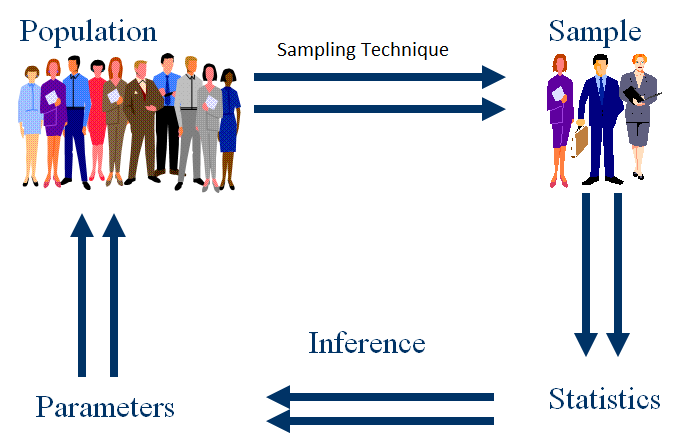
\includegraphics[scale=0.35]{paradigm}
\end{center}
%\textcolor{red}
{Examples of parameters - (true) mean $\mu$, (true) variance $\sigma^2$.\\
Examples of statistics - sample mean $\bar{Y}$, sample variance $S^2=\frac{\sum_{i=1}^{n}(Y_i-\bar{Y})^2}{n-1}$}\\~\\~\\
\textcolor{red}{Inference}
%\underbar{~~~~~~~~~~~~~~~~~~~~~~~~~~~~~}
- Making claims about the population using sample data.

\newpage

\Large \noindent \textbf{Scales (Types) of Data:}\large\\

\begin{itemize}
\item 
\textcolor{red}{\underbar{Qualitative or Categorical}} 
%\underbar{~~~~~~~~~~~~~~~~~~~~~~~~~~~~~~~~~~~~~~}
- A variable that is described by attributes or labels\\
\indent Subscales: \\
Nominal - categories have no ordering (Male, Female)\\
Ordinal - can order categories (Lickert scale data)\\~\\
\item 
\textcolor{red}{\underbar{Quantitative}} 
%\underbar{~~~~~~~~~~~~~~~~~~~~~~~~~~~~~~~~~~~~~~}
- A variable that is described by numerical measurements where arithmetic can be performed\\
\indent Subscales: \\
Discrete - finite or countably infinite \# of values (\# of flowers, 0, 1, 2, ...)\\
Continuous - any value in an interval is possible (Temperature, $(-459.67\deg F, \infty)$)
\end{itemize}

\Large \noindent \textbf{Random Variables and Things of Interest:}\large\\
\begin{itemize}
\item 
\textcolor{red}{\underbar{Random Variable (RV)}} 
%\underbar{~~~~~~~~~~~~~~~~~~~~~~~~~~~~~~~~~~~~~~}
- Numeric outcome to a random process\\~\\
\textbf{Things of interest}\\
\begin{itemize}
\item 
\textcolor{red}{\underbar{Distribution}} 
%\underbar{~~~~~~~~~~~~~~~~~~~~~~~~~~~~~~~~~~~~~~}
- pattern and frequency of observable values\\
For continuous RVs, a smooth curve.  For discrete a `probability histogram.'
\begin{center}
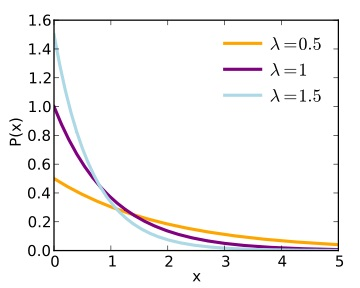
\includegraphics[scale=0.75]{Exponential_pdf}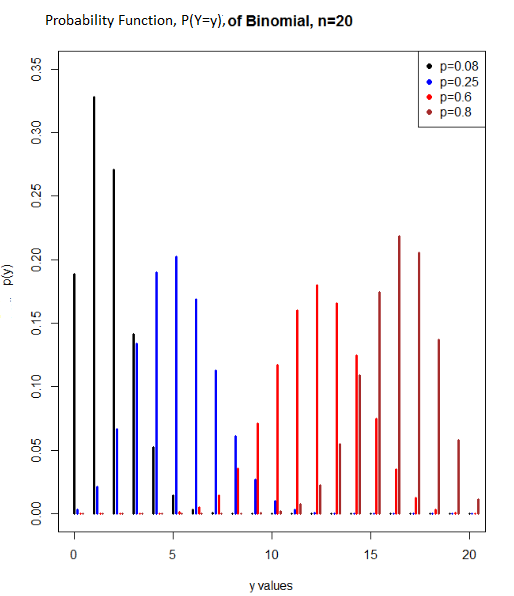
\includegraphics[scale=0.4]{binomialpmf}
\end{center}~\\
\item 
\textcolor{red}{\underbar{Mean/Median}} 
%\underbar{~~~~~~~~~~~~~~~~~~~~~~~~~~~~~~~~~~~~~~~~~~~~~~~~~}
- measures of center of the distribution\\
Main focus often on mean: true mean $\mu$, RV sample mean $\bar{Y}$, observed sample mean $\bar{y}$\\~\\
\item 
\textcolor{red}{\underbar{Standard Deviation, Variance, IQR, Range}} 
%\underbar{~~~~~~~~~~~~~~~~~~~~~~~~~~~~~~~~~~~~~~~~~~~~~~~~}
- measures of spread for the distribution\\
For our purposes, SD and Variance are most important: true variance $\sigma^2$, true SD $\sigma$, observed sample variance $s^2$, observed SD $s$
\end{itemize}
\end{itemize}

\Large \textbf{Graphical Descriptions of RV`s:}\large\\
\begin{itemize}
\item 
\textcolor{red}{\underbar{Histogram}} 
%\underbar{~~~~~~~~~~~~~~~~~~~~~~~~~~~~~~~~~~~~~~~}
- Graphs the frequencies or relative frequencies of realizations of a RV\\~\\
\item 
\textcolor{red}{\underbar{Boxplot}} 
%\underbar{~~~~~~~~~~~~~~~~~~~~~~~~~~~~~~~~~~~~~~~}
- Uses the Five Number Summary ($min,~Q_1,~M,~Q_3,~max$) to display the realizations of a RV
\end{itemize}

\begin{center}
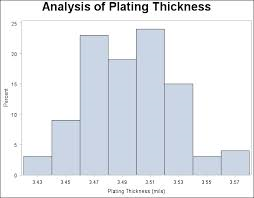
\includegraphics[scale=1]{histogram}~~~~~~~~~~~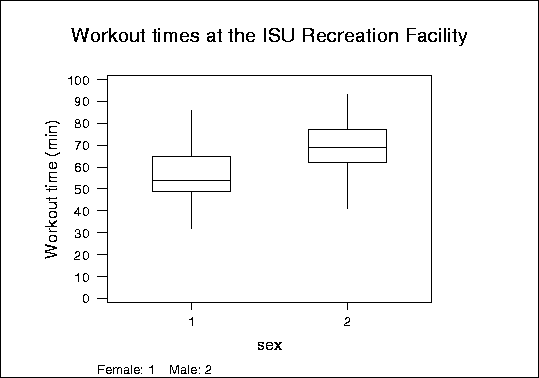
\includegraphics[scale=0.5]{boxplot}
\end{center}

~\\~\\
\Large \textbf{Statistics are RVs!}\large\\~\\
The distribution of a statistic is called a
\textcolor{red}{\underbar{sampling distribution}}\\~\\
%\underbar{~~~~~~~~~~~~~~~~~~~~~~~~~~~~~~~~~~~~~~}\\~\\

We almost always require that our sample is a \textbf{random sample} (RS), or equivalently that our random variables are \textbf{iid} (independent and identically distributed).

\newpage

\textbf{Central Limit Theorem (CLT):}\\~\\
If a RV $Y$ has a (true) mean $\mu$ and (true) variance $\sigma^2$, and a random sample is of size $n\geq 30$ is taken then\\
$$\bar{Y}\sim N(\mu,\sigma^2/n)$$\\
If $Y\sim^{iid} N(\mu,\sigma^2)$ then $\bar{Y}\sim N(\mu,\sigma^2/n)$ for any $n$.\\

\noindent\Large \textbf{Two general methods for inference:}\large\\
\begin{enumerate}
\item 
\textcolor{red}{Confidence Interval (CI)}
%\underbar{~~~~~~~~~~~~~~~~~~~~~~~~~~~~~~~~~~~~~~~~~~~~~~~~~~~~~~~~}
- range of values we believe contain the parameter with some level of confidence\\

\textbf{For an observed $(1-\alpha)100$\% confidence interval $(c_{L}, c_{U})$ we can say}\\~\\
We are $(1-\alpha)100$\% confident the true parameter value is contained in the interval.  (***Do not say probability or chance!)\\

\textbf{The idea of Confidence means}\\~\\
The procedure used to create the interval has a $(1-\alpha)100$\% probability of producing an interval that contains the parameter.\\~\\
i.e. If the experiment were done repeatedly and an interval made for each sample, $(1-\alpha)100$\% of the intervals would contain the parameter value.\\~\\

\item
\textcolor{red}{Hypothesis Test (HT)}
%\underbar{~~~~~~~~~~~~~~~~~~~~~~~~~~~~~~~~~~~~~~~~~~~~~~~~~~~~~~~~}
- test to determine if a given value is reasonable for a parameter\\

\textbf{For a hypothesis test, the p-value means}\\~\\
the probability of observing a test statistic as extreme or more extreme than the one observed, assuming the null hypothesis is true.\\

\textbf{Statistical significance implies}\\~\\
the observed value was unlikely to have occurred by random chance alone (assuming the null hypothesis is true).\\~\\
\end{enumerate}

\Large\textbf{Common ways make inference about $\mu$ (true mean)}:\large\\
\textbf{One sample Z-test}\\
When the true SD, $\sigma$, is known and $\bar{Y}$ has a normal distribution the sampling distribution of the statistic\\
$$Z=\frac{\bar{Y}-\mu}{\sigma/\sqrt{n}} \sim N(0,1)$$
100(1-$\alpha$)\%Ci for $\mu$ is
$$\bar{Y}\pm z_{\alpha/2}\sigma/\sqrt{n}$$
HT: for $H_0:\mu=\mu_0~~vs~~H_A: \mu>\mu_0~~or~~\mu<\mu_0~~or~~\mu\neq\mu_0$
$$\mbox{Test Statistic: }Z=\frac{\bar{Y}-\mu_0}{\sigma/\sqrt{n}}$$
$$RR: \left\{z_{obs}:z_{obs}>z_{\alpha}\right\}~~or~~\left\{z_{obs}:z_{obs}<-z_{\alpha}\right\}~~or~~\left\{z_{obs}:|z_{obs}|>z_{\alpha/2}\right\}$$
$$P-value: P(Z>z_{obs})~~or~~P(Z<z_{obs})~~or~~2*P(Z>|z_{obs}|)$$
~\\

\textbf{One sample T-test}\\
When the true SD, $\sigma$, is unknown we looked at the sampling distribution of the statistic\\
$$T=\frac{\bar{Y}-\mu}{S/\sqrt{n}} \sim t_{n-1}~~\mbox{(valid if RS and Y is normal)}$$
100(1-$\alpha$)\% CI for $\mu$ is
$$\bar{Y}\pm t_{\alpha/2,n-1}S/\sqrt{n}$$
HT: for $H_0:\mu=\mu_0~~vs~~H_a: \mu>\mu_0~~or~~\mu<\mu_0~~or~~\mu\neq\mu_0$
$$\mbox{Test Statistic: } T=\frac{\bar{Y}-\mu_0}{S/\sqrt{n}}$$
$$RR: \left\{t_{obs}:t_{obs}>t_{\alpha,n-1}\right\}~~or~~\left\{t_{obs}:t_{obs}<-t_{\alpha,n-1}\right\}~~or~~\left\{t_{obs}:|t_{obs}|>t_{\alpha/2,n-1}\right\}$$
$$P-value: P(T_{n-1}>t_{obs})~~or~~P(T_{n-1}<t_{obs})~~or~~2*P(T_{n-1}>|t_{obs}|)$$
~\\

\newpage

\noindent\Large \textbf{Inference about two (true) means, $\mu_1$ and $\mu_2$ or $\mu_d=\mu_1-\mu_2$:}\normalsize\\
\textbf{Paired Data:}  (Paired t-test) Assume \textbf{differences} are a RS and normally distributed\\
100(1-$\alpha$)\% CI for $\mu_d$ is
$$\overline{D}\pm t_{\alpha/2,n-1}S_D/\sqrt{n} = \bar{Y}-\bar{X}\pm t_{\alpha/2,n-1}S_{\bar{Y}-\bar{X}}/\sqrt{n}$$
HT: for $H_0:\mu_d=\Delta_0~~vs~~H_a: \mu_d>\Delta_0~~or~~\mu_d<\Delta_0~~or~~\mu_d\neq\Delta_0$
$$\mbox{Test Statistic: } T=\frac{\bar{Y}-\bar{X}-\Delta_0}{S_d/\sqrt{n}}$$
$$RR: \left\{t_{obs}:t_{obs}>t_{\alpha,n-1}\right\}~~or~~\left\{t_{obs}:t_{obs}<-t_{\alpha,n-1}\right\}~~or~~\left\{t_{obs}:|t_{obs}|>t_{\alpha/2,n-1}\right\}$$
$$P-value: P(T_{n-1}>t_{obs})~~or~~P(T_{n-1}<t_{obs})~~or~~2*P(T_{n-1}>|t_{obs}|)$$
~\\
\textbf{Independent Samples:} Assume populations are independent RS's with each population having a normal distribution\\
\textbf{Equal Variance} (Two-sample pooled t-test):\\
100(1-$\alpha$)\% CI for $\mu_d$ is
$$\bar{Y}-\bar{X}\pm t_{\alpha/2,n_1+n_2-2}\sqrt{\frac{(n_1-1)s_1^2+(n_2-1)s_2^2}{n_1+n_2-2}\left(\frac{1}{n_1}+\frac{1}{n_2}\right)}$$
HT: for $H_0:\mu_d=\Delta_0~~vs~~H_a: \mu_d>\Delta_0~~or~~\mu_d<\Delta_0~~or~~\mu_d\neq\Delta_0$
$$\mbox{Test Statistic: } T=\frac{\bar{Y}-\bar{X}-\Delta_0}{\sqrt{\frac{(n_1-1)s_1^2+(n_2-1)s_2^2}{n_1+n_2-2}\left(\frac{1}{n_1}+\frac{1}{n_2}\right)}}$$
$$RR: \left\{t_{obs}:t_{obs}>t_{\alpha,n_1+n_2-2}\right\}~~or~~\left\{t_{obs}:t_{obs}<-t_{\alpha,n_1+n_2-2}\right\}~~or~~\left\{t_{obs}:|t_{obs}|>t_{\alpha/2,n_1+n_2-2}\right\}$$
$$P-value: P(T_{n_1+n_2-2}>t_{obs})~~or~~P(T_{n_1+n_2-2}<t_{obs})~~or~~2*P(T_{n_1+n_2-2}>|t_{obs}|)$$
~\\
\textbf{Unequal Variance} (Two-sample t-test)\\
100(1-$\alpha$)\% CI for $\mu_d$ is
$$\bar{Y}-\bar{X}\pm t_{\alpha/2,\widehat{df}}\sqrt{\frac{s_1^2}{n_1}+\frac{s_2^2}{n_2}}$$
HT: for $H_0:\mu_d=\Delta_0~~vs~~H_a: \mu_d>\Delta_0~~or~~\mu_d<\Delta_0~~or~~\mu_d\neq\Delta_0$
$$\mbox{Test Statistic: } T=\frac{\bar{Y}-\bar{X}-\Delta_0}{\sqrt{\frac{s_1^2}{n_1}+\frac{s_2^2}{n_2}}}$$
$$RR: \left\{t_{obs}:t_{obs}>t_{\alpha,\widehat{df}}\right\}~~or~~\left\{t_{obs}:t_{obs}<-t_{\alpha,\widehat{df}}\right\}~~or~~\left\{t_{obs}:|t_{obs}|>t_{\alpha/2,\widehat{df}}\right\}$$
$$P-value: P(T_{\widehat{df}}>t_{obs})~~or~~P(T_{\widehat{df}}<t_{obs})~~or~~2*P(T_{\widehat{df}}>|t_{obs}|)$$
$$\widehat{df}=\frac{\left(\frac{s_1^2}{n_1}+\frac{s_2^2}{n_2}\right)^2}{\left(\frac{s_1^2}{n_1}\right)^2/(n_1-1)+\left(\frac{s_2^2}{n_2}\right)^2/(n_2-1)}$$

\newpage

\noindent\Large \textbf{Extension of two-sample pooled t-test to inference about t (true) means, $\mu_1, \mu_2, ..., \mu_t$:}
\large\\
Analysis used for a completely randomized design.  \\~\\
One Way ANOVA model:\\
$$Y_{ij}=\mu_{i}+E_{ij}$$
where $E_{ij}\sim^{iid}N(0,\sigma^2)$, $i=1,2,...t$, and $j=1,2,...,n$ (total sample size = $nt=N$)\\~\\
$\mu_{i}$ is the mean for group $i$ and $\sigma^2$ is the common variance for each population.\\~\\
An alternative model:
$$Y_{ij}=\mu+\tau_{i}+E_{ij}$$
where $\mu$ is the overall (grand) mean, $\tau_i$ is the effect for the $i^{th}$ treatment, and $E_{ij}\sim^{iid}N(0,\sigma^2)$

Data and labeling:  
\normalsize
\begin{center}
\begin{tabular}{cc|cc}
Corn Syrup & Replicate \# & `L' measurement  & Label\\\hline
26 &1& 51.89&$y_{11}$\\
26 &2& 51.52&$y_{12}$\\
26 &3& 52.69&$y_{13}$\\
42 &1& 47.21&$y_{21}$\\
42 &2& 48.57&$y_{22}$\\
42 &3& 47.57&$y_{23}$\\
55 &1& 41.43&$y_{31}$\\
55& 2& 42.31&$y_{32}$\\
55& 3& 42.31&$y_{33}$\\
\end{tabular}
\end{center}

\large
Balanced One-way ANOVA table (same number of replicates per group)\\
\begin{center}
\begin{tabular}{c|c|c|c|c|c}
Source & DF & SS & MS & F-stat & P-value\\
\hline& & & & &\\
Treatment & $t-1$ & $n\sum_{i=1}^{t}(\bar{Y}_{i\bullet}-\bar{Y}_{\bullet\bullet})^2$ & $\frac{SS(Trt)}{t-1}$ & $\frac{MS(Trt)}{MS(E)}$ & Use $F(t-1,t(n-1))$\\& & & & &\\
Error & $t(n-1)$ & $\sum_{i=1}^{t}\sum_{j=1}^{n}(Y_{ij}-\bar{Y}_{i\bullet})^2$ & $\frac{SS(E)}{t(n-1)}$ &  & \\& & & & &\\
Total & $nt-1$ & $\sum_{i=1}^{t}\sum_{j=1}^{n}(Y_{ij}-\bar{Y}_{\bullet\bullet})^2$ & & & \\
\end{tabular}
\end{center}

~\\~\\
P-value from ANOVA table tests 
$$H_0: \mu_1=\mu_2=...=\mu_t\mbox{  vs  }H_A: \mbox{at least 1 mean differs}$$
